\documentclass{article}% For the example only, any class will do

\usepackage{tikz}
\usetikzlibrary{positioning}% To get more advances positioning options
\usetikzlibrary{arrows,automata}% To get more arrow heads

\begin{document}

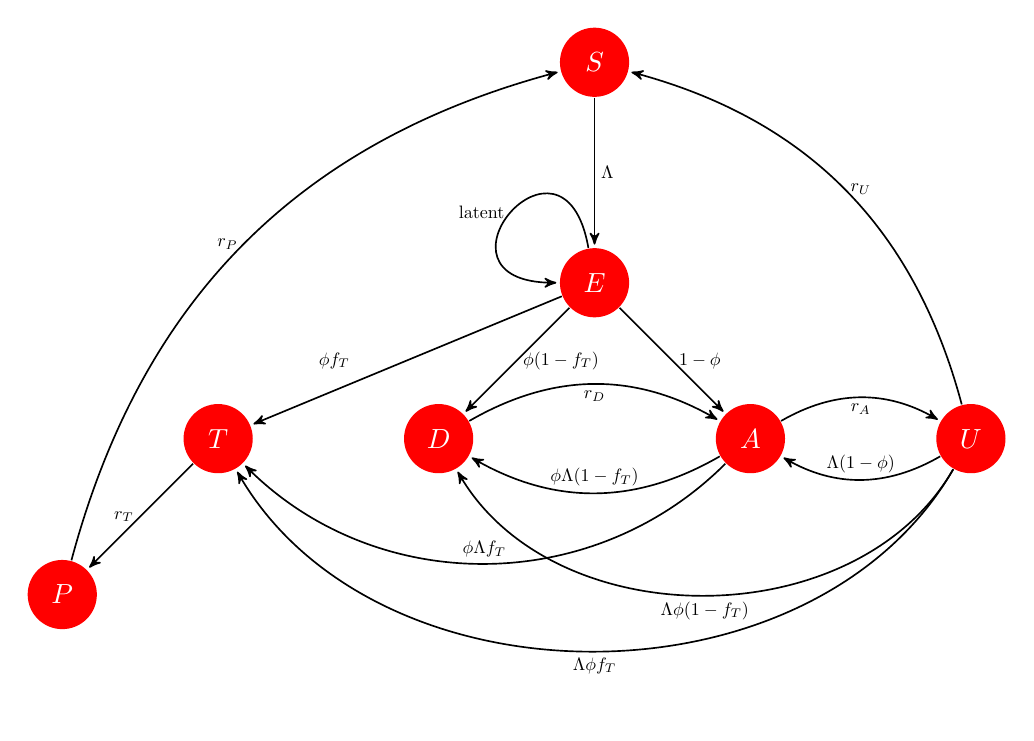
\begin{tikzpicture}[->,>=stealth',shorten >=1pt,auto,node distance=2.8cm,
                    semithick]
  \tikzstyle{every state}=[fill=red,draw=none,text=white]

  \node[state] 	     (S)                    {$S$};
  \node[state]         (E) [below of=S] {$E$};
  \node[state]         (D) [below left of=E] {$D$};
  \node[state]         (T) [left of=D] {$T$};
  \node[state]         (A) [below right of=E] {$A$};
  \node[state]         (U) [right of=A] {$U$};
  \node[state]         (P) [below left of=T] {$P$};
  
\begin{scope}[every node/.style={scale=.65}]

\draw (S) to node [right] {$\Lambda$} (E);
\draw (E) to [out=100,in=180,looseness=8,left] node {latent} (E);
\draw (E) to node [left=0.25in] {$\phi f_{T}$} (T);
\draw (E) to node [right] {$\phi(1-f_{T})$} (D);
\draw (E) to node [right] {$1-\phi$} (A);
\draw (D) edge [bend left] node [below] {$r_{D}$} (A);
\draw (A) edge [bend left] node [above] {$\phi\Lambda (1-f_{T})$} (D);
\draw (A) edge [bend left=45] node [above] {$\phi\Lambda f_{T}$} (T);
\draw (A) edge [bend left] node [below] {$r_{A}$} (U);
\draw (U) edge [bend left] node [above] {$\Lambda (1-\phi)$} (A);
\draw (U) edge [bend left=60] node [below] {$\Lambda\phi(1-f_{T})$} (D);
\draw (U) edge [bend left=60] node [below] {$\Lambda\phi f_{T}$} (T);
\draw (U) edge [bend right] node [right] {$r_{U}$} (S);
\draw (T) to node [left] {$r_{T}$} (P);
\draw (P) edge [bend left] node [left] {$r_{P}$} (S);

\end{scope}

\end{tikzpicture}

\end{document}